The use of transition metals for cancer treatment started in the year 1960 when Dr. Barnett Rosenberg discovered cis-diammine-dichloroplatinum (II) (cisplatin) showed anti-tumor activity \cite{rosenberg1965inhibition}. Other transition metals, including but not limited to copper, rhodium ,ruthenium, zinc, iron, and palladium, also exhibit anti-cancer properties \cite{rafique2010transition}. In this section, we study several of these anti-cancer agents. Effectiveness of anti-tumor compounds are measured by the inhibitory concentrations (IC\textsubscript{50})  values. The compounds exhibited IC\textsubscript{50} activity within the range of 10–\SI{25}{\micro}g ml$^{-1}$ are considered weak anticancer drugs, while those of IC\textsubscript{50} activity between 5 and \SI{10}{\micro}g ml$^{-1}$ are moderate and compounds of activity below \SI{5}{\micro}g ml$^{-1}$ are considered strong antitumour agents \cite{mansour2016flubendazole}.


\begin{figure}[!ht]
        \centering
        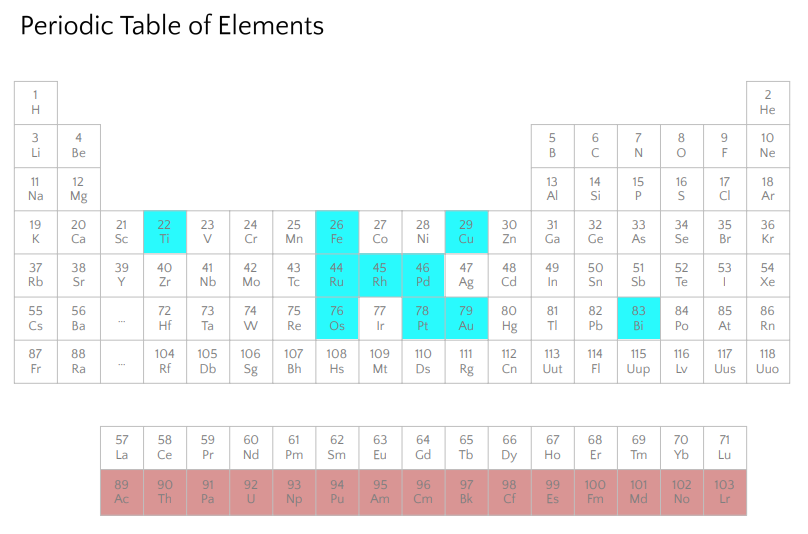
\includegraphics[scale = 0.55]{periodictable.png}
        \caption{Transition metals used as anti-cancer agents (highlighted blue) \cite{rafique2010transition}}
        \label{fig:transition}
      \end{figure}
      
\subsection{Platinum Complexes}
Cisplatin is the first transition metal complex used to treat various cancers, including bladder, testicular, ovarian, lung, and head cancers\cite{dilruba2016platinum}. 

\hspace{0.1cm}Cisplatin affects specific common tissues found in the hair follicle, bone marrow, and gastrointestinal lining tract. Cisplatin affects the growth of these cells that have been affected by cancer \cite{rafique2010transition}. In chemotherapy, the patient is administered cisplatin through the blood. In the blood, the chloride concentration is high, and hence the cisplatin remains in neutral form. Upon entering a cell, Chloride ion concentration drops, and the cisplatin goes and attaches with the DNA. The cell's nuclear proteins, such as high mobility group-domain (HMG) proteins, identify these cisplatin-DNA connections and protect the cell they begin to perform repair, finally leading to the cell's death \cite{shaili2014platinum}. While cisplatin certainly proved useful in treating cancerous cells, it had one major drawback, which drugs often face, known as `Drug Resistance'. The cancerous cells developed resistance to cisplatin and other Pt(II) complexes due to mutations. Cisplatin showed other side effects, including - nephrotoxicity, nausea, renal toxicity, vomiting, hair loss, and asthenia \cite{boulikas2007molecular}. To tackle these drawbacks, the second and third generation of platinum drugs such as carboplatin and other related drugs came into use.

\begin{figure}[!ht]
    \centering
    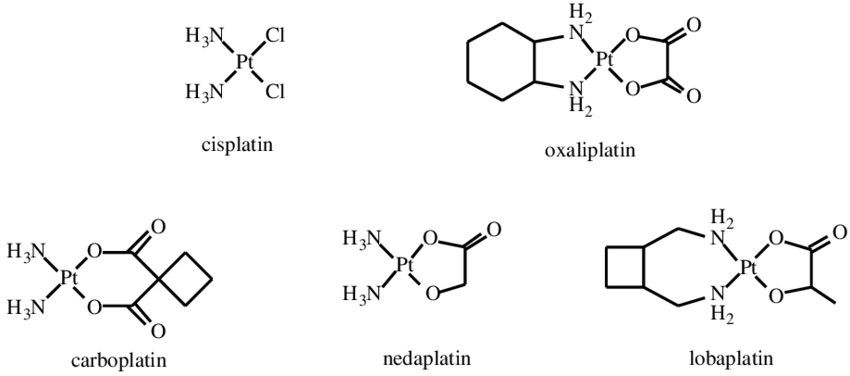
\includegraphics[scale = 0.55]{cisplatin.png}
    \caption{Various platinum complexes used as anti-cancer Drugs}
    \label{fig:cisplatin}
\end{figure}

\hspace{0.1cm}These second and third-generations of platinum drugs have different leaving groups and varying amines\cite{shaili2014platinum}. Figure \ref{fig:cisplatin} shows examples of these drugs - carboplatin, oxaliplatin, nedaplatin, and lobaplatin. They worked similarly except with lesser side effects and minor toxicity. Hence they're a viable option in high-dosage treatment. Carboplatin is used for treating the same variety of cancers as cisplatin, whereas oxaliplatin is mainly used in treating colorectal cancer\cite{kelland2007resurgence}. Even with reduced side effects, these drugs still could not overcome the `Drug Resistance' problem. Nedaplatin also has reduced toxicity and is used primarily for small cell lung cancer (SCLC) and head and neck cancer\cite{dilruba2016platinum}. 

\hspace{0.1cm}To further reduce the toxicity and the drug resistance problem of these second and third-generation drugs, a new strategy using Pt (IV) complexes as prodrugs came into development. A prodrug is a drug that isn't active when administered and becomes operational later in the body. Pt(IV) complexes allow for two additional ligands compared to Pt(II) complexes, and hence they have different chemical properties. Pt(IV) complexes are kinetically inert, making sure that the drug remains inactive en route to the tissues. Finally, after entering the cells, these Pt(IV) complexes get reduced to Pt(II). The main idea behind these complexes' activation is to use light to photoactivate them, which leads us to photodynamic therapy (PDT) \cite{dilruba2016platinum}. Figure \ref{fig:prodrugs} shows examples of a few Pt(IV) complexes used as prodrugs. PDT includes activation of a photosensitizer (PS) using a suitable wavelength and intensity of light. Photodynamic reaction (PDR) is the excitation of the PS in the presence of oxygen. The PR then causes changes in the cell leading to apoptosis of the tumor \cite{allison2013photodynamic}. PDT wasn't effective as it caused tumor-associated hypoxia, which in turn was responsible for drug resistance \cite{liu2017chemical}.


\begin{figure}[!ht]
    \centering
    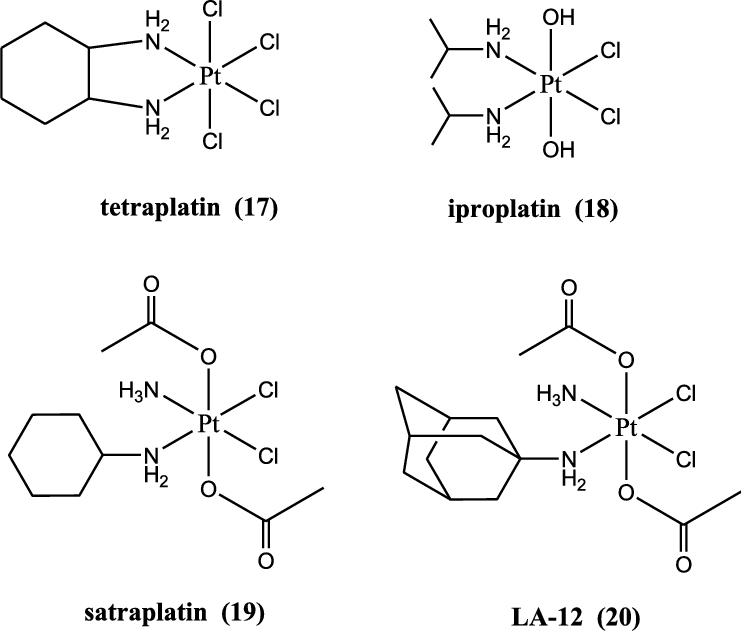
\includegraphics[scale = 0.35]{prodrugs.png}
    \caption{Pt(IV) Complexes used as prodrugs}
    \label{fig:prodrugs}
\end{figure}
\hspace{0.1cm}We now explore recent developments of Platinum complexes in the field of chemotherapy. Guo et al.  \cite{guo2018platinum} proposed the use of a Pt(IV) complex in combinatorial chemo-photodynamic therapy. The authors used the Pt(IV) complex and observed that it produces the highly toxic Pt(II) inside the cell and doesn't require a PS and oxygen for conversion of Pt(IV) to Pt(II). The authors synthesized a platinum(IV) complex-based prodrug monomer (PPM) containing symmetrical axial bis-urethan ethyl methacrylate ligands. Further, they confirmed that this Pt(IV) species is easily converted to Pt(II) without using a PS and oxygen; this tackles the hypoxia dilemma. To make the delivery of the complex easier, they copolymerize the PPM with 2-methacryloyloxyethyl phosphorylcholine (MPC) monomer, and this increases biocompatibility, solubility, and blood circulation time. The authors show that the drug worked effectively in mice and successfully suppressed cancer cells with good efficacy. Guo et al. \cite{guo2017prodrug} proposed a nanoparticle-based approach that consists of photosensitizer, angiogenesis vessel targeting peptide, and bioreductive prodrug for chemo-photo synergistic cancer therapy. The authors use the state of hypoxia of the cell to activate the bioreductive prodrug for chemo-photo tumor suppression. This procedure proved useful in mouses. 

\hspace{0.1cm}In general the various new methods that use platinum complexes involve modification to the method of delivery to reduce the toxic profile, conjugation with bioactive molecules, introduction of axial ligands, and merging two or more platinum coordination spheres.

\subsection{Bismuth Complexes}
In general, bismuth has unusually low toxicity when compared to tin and lead. Therefore compounds of bismuth are generally considered medicinally safe for use. Bi(III) readily forms complexes with ligands bearing oxygen, nitrogen, and sulphur donor atoms, making them fit for biological systems. Researchers had observed that bismuth complexes had shown anti-microbial properties and hence were useful in a medicinal context.
\hspace{0.1cm}Recently researchers gained insight into its anti-cancer properties too. \ce{^{212} Bi} and \ce{^{213} Bi} are radioactive. They emit alpha and beta particles. They have a short-range penetration power (50–\SI{80}{\micro\metre}), which causes lesser damage to the surrounding non-cancerous cells\cite{yang2007biocoordination}. The first tested bismuth anti-tumor compound was the bismuth complex with 6-mercaptopurine, but it was never used in the treatment because of it's low solubility. The Figure \ref{fig:bismuth} shows the method of preparation of this complex. Ligands used in bismuth complexes include thiosemicarbazones, hydrazones, and dithiocarbamates, as they have shown anti-cancer properties \cite{kowalik2019recent}.
\begin{figure}[!ht]
    \centering
    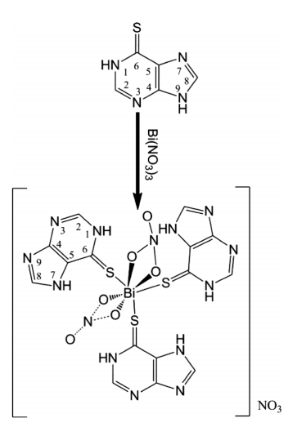
\includegraphics[scale = 0.85]{bismuth.png}
    \caption{\ce{[Bi(MP)3(NO3)2]NO3}}
    \label{fig:bismuth}
\end{figure}
Ouyang et al. \cite{ouyang2017potent} proposed  bismuth(III) complex derived from pentadentate-2,6-pyridinedicarboxaldehyde bis(4 N-methylthiosemicarbazone), \ce{[BiL(NO3)2]NO3} [L = 2,6-pyridinedicarboxaldehyde bis(4 N-methylthiosemicarbazone)]. The authors showed that this new \ce{[BiL(NO3)2]NO3} considerably inhibited the formation of the affected colony (ranging from 10 to 15\%), migration of the tumor and remarkably caused apoptosis (ranging from 18.69 to 20.03\% for the mid-late apoptosis) of human lung cancer cells -  A549 and H460. The authors conducted in vivo studies that indicated that tumor-affected mice treated with \ce{[BiL(NO3)2]NO3} effectively inhibited A549 xenograft tumor growth. There were no noticeable effects on the mice. 

\hspace{0.1cm}Ferreira et al. \cite{ferreira2016bismuth} explored Bismuth(III) complexes with 2-acetylpyridine- and
2-benzoylpyridine-derived hydrazones. It was observed that  the 2-benzoylpyridine derived hydrazones proved to be less potent as cytotoxic agents, and less selective than the corresponding 2-acetylpyridine derivatives for bismuth (III) complexes. Song et al. \cite{song2016perfluorocarbon} suggested the use of Perfluorocarbon-loaded hollow Bi2Se3 nanoparticles for enhancing radiotherapy (RT) by overcoming hypoxia-associated RT resistance. The authors use Bi2Se3 nanoparticles, that are easily prepared
by a facile cation exchange method and then functionalized with
polyethylene glycol (PEG). The hollow structure of the particle allows for fluorohexane to be fit perfectly, which can then act as a oxygen reservior overcoming the hypoxia problems. This way the cancer affected cell is offered more radiation and hence there is a higher probability of the death of the cell. This technique is effective in the case of deeply located tumors that maybe not be accessible to light easily and hence NIR, X-ray or ultrasound could be used to trigger it. Although Bismuth complexes are not toxic in nature, several side effects have been observed - dizziness, loss of taste, abdominal pain and a very few patients have been found to have parageusia and glossitis\cite{yang2015bismuth}.


\begin{table}[]
\centering
 \begin{tabular}{ |p{0.25\linewidth}|p{0.25\linewidth}|p{0.45\linewidth}|} 
  \hline
  Author & IC$_{50}$  Value & Summary\\ \hline
  Marzano et al. \cite{marzano2013crystal} & \SI{44}{\micro\metre} against myelogenous leukemia cells & implying more potent anticancer effects than the free ligand \\ \hline
  Li et al \cite{li2012nine}& \SI{26.8}{\micro\metre} against K562 leukemia cells &  A nine-coordinate bismuth(III) complex derived from pentadentate 2,6-diacetylpyridine bis-(N-methylthiosemicarbazone) showed much
  higher antibacterial and anticancer activities than its parent ligand \\ \hline
  Zhang et al. \cite{zhang2012synthesis}& \SI{1.6}{\micro\metre} & 2-acetylpyrazine-N (4)-pyridylthiosemicarbazone and its bismuth (III) complex shoed anti-cancer properties\\ \hline
  Islam et al. \cite{islam2016cytotoxicity}& \SI{3.0}{\micro\metre} against K562 cell& \ce{Ph3Bi(2AcB)2} is used\\ \hline
  Islam et al. \cite{islam2016cytotoxicity}& \SI{19.6}{\micro\metre} against K562 cell& \ce{Ph3Bi(4AcB)2} is used \\ \hline
  \end{tabular}
\newline
\\
 \caption{Various Bi complexes indicating anti-tumor activity compared with respect to their IC$_{50}$ Value, which refers to  compound concentration that produces $50\%$ of cell death; K562 -  chronic myelogenous leukemia}
\label{tab:bimethods}
\end{table}

\subsection{Palladium Complexes}
Palladium is the element right above Platinum. Since Pt complexes proved to be effective, Pd complexes also began to be explored as potential chemotherapeutic agents. Pd(II) complexes show similar coordination chemistry when compared to Pt(II) complexes. The significant difference is that the Pd(II) complexes have better solubility and kinetic liability than Pt(II) complexes \cite{garoufis2009palladium}.

\begin{figure}[!ht]
    
    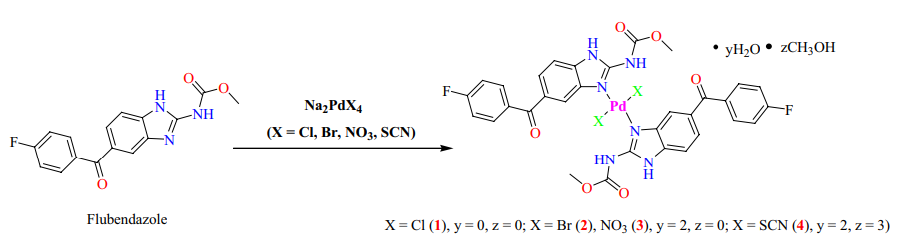
\includegraphics[scale = 0.775]{palladium.png}
    \caption{The synthesized Flubendazole Pd(II) complexes}
    \label{fig:palladium}
\end{figure}

\hspace{0.1cm} Mansour et al. \cite{mansour2016flubendazole} synthesized Flubendazole(FLU) Pd(II) complexes as the benzimidazole moiety, and its derivatives are known to have anti-tumor properties. Benzimidazole can serve as a monodentate ligand or as a bridge, forming various polynuclear complexes. The authors tested the synthesized compounds for anti-tumor properties against n human breast cancer, hepatocarcinoma, and colon carcinoma cells.  The solid Pd(II) complexes of FLU [X = Cl (1), Br (2), \ce{NO3} (3), and SCN (4)] as shown in the Table \ref{tab:pdm}, changing `X' leads to different cytotoxic activity. They studied the structural properties of Flubendazole Pd(II) complexes, and they observed that E\textsubscript{HOMO}, energy gap, and dipole moment were the most significant descriptors for the correlation with the anti-tumor activity. 

\begin{table}[]
\centering
\begin{tabular}{|c|c|}
\hline
X   & IC\textsubscript{50} value (\SI{}{\micro}g ml$^{-1}$) \\ \hline
Cl  & 4.13               \\ \hline
Br  & 3.53               \\ \hline
\ce{NO3} & 3.68               \\ \hline
SCN & 3.68               \\ \hline
\end{tabular}
\caption{IC50 values of the compounds with different `X' molecules}
\label{tab:pdm}
\end{table}

\hspace{0.1cm} Ayyannan et al. \cite{ayyannan2016design} synthesized New palladium(II) complexes \ce{[Pd(L)(PPh3)]} and \ce{[Pd(L)(AsPh3)]} (Figure \ref{fig:pdtwo} shows the synthesis and structure of the complexes)using 4-hydroxy benzoic acid (5-chloro-2-hydroxy-benzylidene)-hydrazide (\ce{H2L}) ligand  (Figure \ref{fig:pdone} shows the synthesis of the ligand). These complexes' structure is square planar with the hydrazone coordinated through ONO atoms was confirmed using analytical, spectral, and single-crystal X-ray diffraction techniques. Analysis of the complexes' cytotoxicity in vitro cleared showed high activity levels against human cervical (HeLa) and breast (MCF-7) cancer cells. \ce{[Pd(L)(PPh3)]} complex showed higher cytotoxicity than \ce{[Pd(L)(AsPh3)]} complex, potentially because of better binding ability. Triphenylphosphine as co ligand led to increased interaction with DNA/BSA, free radical, and tumor cell line than the rest of the ligand and complex.

\begin{figure}[!ht]
    \centering
    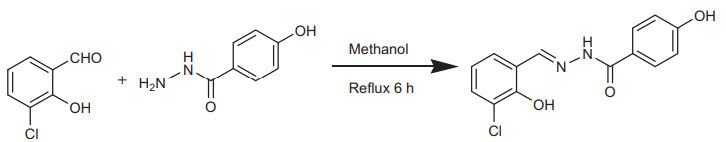
\includegraphics[scale = 0.75]{pdone.png}
    \caption{Synthesis of hydrazone ligand}
    \label{fig:pdone}
\end{figure}

\begin{figure}[!ht]
    \centering
    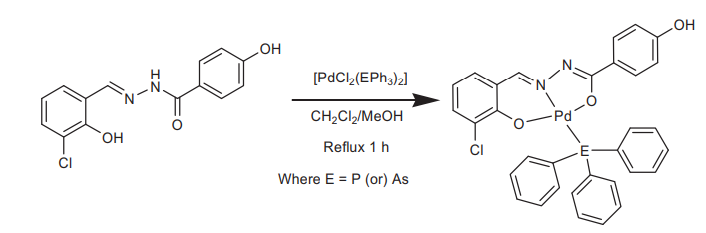
\includegraphics[scale = 0.75]{pdtwo.png}
    \caption{Synthesis of the palladium(II) complexes \cite{ayyannan2016design}}
    \label{fig:pdtwo}
\end{figure}

\begin{table}[]
\centering
\begin{tabular}{|c|c|c|}
\hline
Compounds & IC\textsubscript{50} value \SI{}{\micro}M & Type of cancer         \\ \hline
\ce{[Pd(L)(PPh3)]}        & 18.92           & \multirow{3}{*}{HeLa}  \\ \cline{1-2}
\ce{[Pd(L)(AsPh3)]}        & 24.63           &                        \\ \cline{1-2}
Cisplatin & 16.21           &                        \\ \hline
\ce{[Pd(L)(PPh3)]}       & 18.65           & \multirow{3}{*}{MCF-7} \\ \cline{1-2}
\ce{[Pd(L)(AsPh3)]}       & 31.74           &                        \\ \cline{1-2}
Cisplatin & 15.35           &                        \\ \hline
\end{tabular}
\caption{IC50 values of the Pd complexes in comparison to cisplatin}
\label{tab:pdcomplexes}
\end{table}

\begin{figure}[!ht]
    \centering
    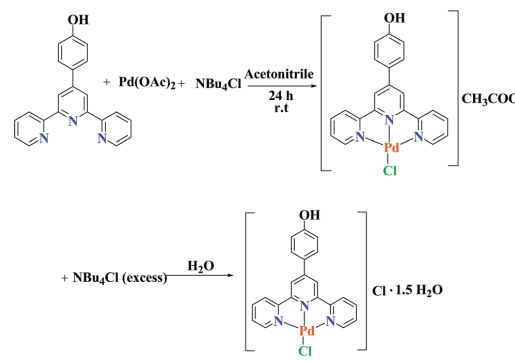
\includegraphics[scale = 0.75]{pdthree.png}
    \caption{Synthesis of the palladium(II) complexes}
    \label{fig:pdthree}
\end{figure}

\hspace{0.1cm}Rodi\'c et al. \cite{rodic2016synthesis} studied and synthesized three copper(II) complexes with N2O ligand di(2-pyridil) ketone 1-adamantoyl hydrazone (Addpy) of the formula \ce{[CuII 2CuI 2(Addpy)2Br2(m-Br4)]}, catena-poly\ce{[CuCl(m-Addpy)(m-Cl)CuCl2]n} and \ce{[Cu(Addpy)(NCS)2]}. The authors observed that these copper(II) complexes have remarkable anti-cancer properties and were tested against HeLa, colorectal carcinoma (LS174), lung cancer (A549), leukemia (K562), and adenocarcinoma (MDA-MB231) cancer cell lines. 
Table \ref{table:copperone} compares the value of cisplatin to the copper(II) complexes as proposed by the authors. 

\begin{table}[!ht]
    \centering
    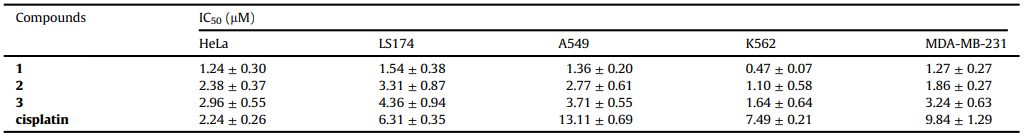
\includegraphics[scale = 0.65]{copperone.png}
    \centering
    \caption{IC\textsubscript{50} values comparison.\\ 
    1 - \ce{[CuII 2CuI 2(Addpy)2Br2(m-Br4)]}, \\
    2 - \ce{[CuCl(m-Addpy)(m-Cl)CuCl2]n}, 3 - \ce{[Cu(Addpy)(NCS)2]}}
    \label{table:copperone}
\end{table}

\subsection{Copper Complexes}
Copper is a biologically quintessential element, and it plays roles in normal human metabolism and the advancement of anti-tumor agents \cite{rajalakshmi2014dna}.

\hspace{0.1cm}Lewis et al. \cite{lewis2016chemical} explored the biological properties of two Cu(II) complexes with imidazole or thiazole-containing ligands. Complex 1, \ce{[Cu(PyBIm)(NO3)(H2O)](NO3)}, is a four coordinate, distorted square planar species with one ligand (N,N), nitrate, and water bound to Cu(II). The \ce{[Cu(PyBIm)3](BF4)2} complex (2) has distorted octahedral geometry with a 3:1 Py(BIm) ligand to metal ratio. The distorted trigonal bi-pyramidal geometry of compound 3, \ce{[Cu(PyBTh)2(H2O)](BF4)2}, is comprised of two PyBTh ligands and one water. The authors investigated the anti-cancer properties of these complexes against HeLa or K562 cells. Figure \ref{fig:coppertwo} shows the method of preparation of these Cu(II) complexes.

\begin{figure}[!ht]
    \centering
    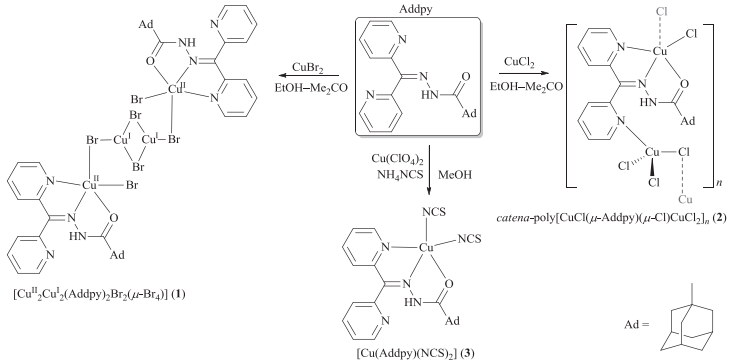
\includegraphics[scale = 0.75]{coppertwo.png}
    \caption{Synthetic routes for \ce{[Cu(PyBIm)(NO3)(H2O)](NO3)} (1), \ce{[Cu(PyBIm)3](BF4)2} (2), and \ce{[Cu(PyBTh)2(H2O)](BF4)2} (3)}
    \label{fig:coppertwo}
\end{figure}

\begin{table}[]
\centering
\begin{tabular}{|c|c|c|}
\hline
Compounds & IC\textsubscript{50} value \SI{}{\micro}M & Type of cancer         \\ \hline
\ce{[Cu(PyBIm)(NO3)(H2O)](NO3)} & 2.5 ± 1.5 & \multirow{3}{*}{HeLa} \\ \cline{1-2}
\ce{[Cu(PyBIm)3](BF4)2} & 2.4 ± 1.4 &                       \\ \cline{1-2}
\ce{[Cu(PyBTh)2(H2O)](BF4)2} & 7.7 ± 2.4 &                       \\ \hline
\ce{[Cu(PyBIm)(NO3)(H2O)](NO3)} & 2.3 ± 0.8 & \multirow{3}{*}{K562} \\ \cline{1-2}
\ce{[Cu(PyBIm)3](BF4)2} & 5.0 ± 0.5 &                       \\ \cline{1-2}
\ce{[Cu(PyBTh)2(H2O)](BF4)2} & 4.6 ± 0.8 &                       \\ \hline
\end{tabular}
\caption{IC50 values of the Pd complexes in comparison to cisplatin}
\label{tab:pdcomplexes}
\end{table}

\hspace{0.1cm}Kilian et al. \cite{kilian2016fast} proposed using the Cu-porphyrin complex for positron emission tomography (PET) imaging. In general, porphyrin-based photosensitizers are useful in photodynamic therapy and fluorescence imaging of cancer. TCPP is the porphyrins that have the ability to chelate the metal ion. The reason to use the Cu-porphyrin complex is that the decay characteristics of the $^64$Cu isotope. The authors present a method for the synthesizing Cu(II)-TCPP useful in the PET, especially short-lived $^60$Cu and $^62$Cu. 

\begin{figure}[!ht]
    \centering
    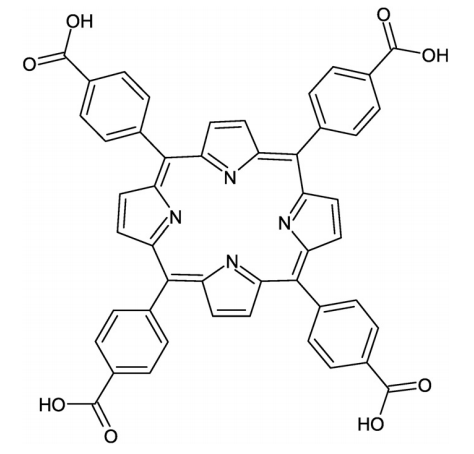
\includegraphics[scale = 0.5]{copperthree.png}
    \caption{Strcuture of TCPP}
    \label{fig:copperthree}
\end{figure}


\subsection{Iron Complexes}
\hspace{0.1cm}Currently, iron complexes are being developed to fight tumors partly because of their two oxidation states that are Fe(II) and Fe(III), the ability of iron to transform from one to the other and, in the process, either lose or accept an electron has a significant impact on a vast majority of biological functions \cite{fairweather2004iron}. The two first iron complexes investigated and discovered to have anti-cancer properties are ferrocenium picrate and ferrocenium trichloroacetate complexes. The anti-cancer properties of these salts stemmed from the fact that ROS formation is observed, which leads to oxidative DNA damage \cite{kopf1984ferricenium}. The Figure \ref{fig:ironone} shows the strcuture of ferrocenium picrate and ferrocenium trichloroacetate.

\begin{figure}[!ht]
    \centering
    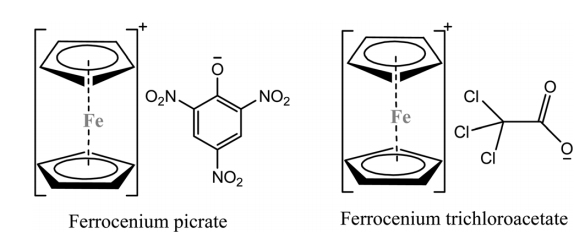
\includegraphics[scale = 0.55]{ironone.png}
    \caption{Strcuture of ferrocenium picrate and ferrocenium trichloroacetate}
    \label{fig:ironone}
\end{figure}

\hspace{0.1cm}Estrada-Montaño et al.\cite{estrada2017iron} studied the Iron(III) Pincer Complexes for their anti-cancer properties. \ce{[Fe(NCN)2]PF6} (1·PF6) [NCHN = 1,3-di(pyridin-2- yl)benzene] was easily obtained by a transmetalation reaction between \ce{[Fe3(CO)12]} and \ce{Hg(NCN)Cl}. The proposed structure was verified using  X-ray diffraction, electron paramagnetic resonance spectroscopy, and cyclic voltammetry. The authors measured the cytotoxicity against human colon cancer (HCT-15), lung cancer (SKLU), and gastric cancer (AGS, KATOIII) cell lines by determining the IC\textsubscript{50} values. The IC\textsubscript{50} values clearly indicated these complexes as being more effective than cisplatin.

\hspace{0.1cm}Xie et al. \cite{xie2017anticancer} examined Fe(II) complexes with phenanthroline derivatives as ligands and their anti-cancer properties. The complexes synthesized include -  \ce{[Fe(II)(pip)3]}$^{2+}$, \ce{[Fe(II)(pip-CH3)3]}$^{2+}$, \ce{[Fe(II)(pip-OCH3)3]}$^{2+}$, \ce{[Fe(II)(pip-NO2)3]}$^{2+}$, \ce{[Fe(II)(pip-COOH)3]}$^{2+}$, \ce{[Fe(II)(pip-OH)3]}$^{2+}$. Among these complexes \ce{[Fe(II)(pip-OCH3)3]}$^{2+}$ has insignificant toxicity, and the reason for the death of cancer cells is apoptosis. The Figure \ref{fig:ironthree} shows the aforementioned complexes.

\begin{figure}[!ht]
    \centering
    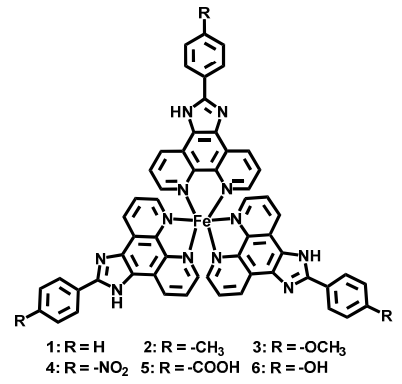
\includegraphics[scale = 0.7]{ironthree.png}
    \caption{Strcuture of Fe(II) complexes with phenanthroline derivatives}
    \label{fig:ironthree}
\end{figure}

\subsection{Ruthenium Complexes}
Ruthenium complexes are prominent in medicinal chemistry as anti-tumor agents because of particular antimetastatic properties and low systemic toxicity. Ruthenium compounds seem to penetrate the tumor cells to a reasonable extent and effectively bind to the DNA. The anti-tumor activity of ruthenium complexes is associated with the binding of these complexes to the DNA. These ruthenium complexes form adducts with DNA that block DNA and RNA synthesis and induce the infected cell's death. With particular attention to their electron-transfer properties, the chemistry of ruthenium complexes has remained quite active for the latest decades. Ruthenium offers a wide range of oxidation states which are easily accessible chemically and electrochemically (from oxidation state -2 in \ce{[Ru(CO)4]} 2- to +8 in \ce{RuO4}); this is what makes the complexes of ruthenium redox-active \cite{kostova2006ruthenium}.

\hspace{0.1cm}Lazić et al. \cite{lazic2016dna} studied and synthesized ruthenium(II) terpyridine complexes, i.e., \ce{[Ru(Cl-tpy)(en)Cl][Cl]} and \ce{[Ru(Cl-tpy)(dach)Cl][Cl]}. The authors reported that ethylenediamine is instrumental for the ruthenium(II) terpyridine complexes' cytotoxic activity. This study presents further confirmation that ruthenium complexes could have multiple targets and mechanisms of action. Table \ref{tab:ruth} shows the IC\textsubscript{50} values of the ruthenium(II) terpyridine complexes.


\begin{table}
\begin{tabular}{|l|l|l|l|} 
\hline
\multirow{2}{*}{Ruthenium~complex}               & \multicolumn{3}{l|}{IC50 values [\SI{}{\micro}M]}           \\ 
\cline{2-4}
                                                 & A549            & HCT116       & ~CT26          \\ 
\hline
\ce{[Ru(Cl-tpy)(en)Cl][Cl]}   & 58.40 ± 0.10~~  & 66.30 ± 0.20 & 32.80 ± 0.10   \\ 
\hline
\ce{Ru(Cl-tpy)(dach)Cl][Cl]} & 110.80 ± 0.30~~ & 84.40 ± 0.10 & 72.80 ± 0.20~  \\ 
\hline
Cisplatin                                        & 33.00 ± 0.10~~  & 45.10 ± 0.20 & 24.70 ± 0.10   \\
\hline
\end{tabular}
\caption{IC50 values of ruthenium(II) terpyridine complexes}
\label{tab:ruth}
\end{table}

Zhang et al. \cite{zhang2016synthesis} synthesized and investigated four new ruthenium(II) polypyridyl complexes \ce{[Ru(dmb)2(DQTT)](ClO4)2} 
(DQTT = 12-(1,4- dihydroquinoxalin-6-yl)-4,5,9,14-tetraazabenzo[b]triphenylene, dmb = 4,4′-dimethyl-2,2′-bipyridine), \\ \ce{[Ru(bpy)2(DQTT)](ClO4)2} (bpy = 2,2′-bipyridine), \\ \ce{[Ru(phen)2(DQTT)](ClO4)2} (phen = 1,10- phenanthroline) \\ and \ce{[Ru(dmp)2(DQTT)](ClO4)2} \\ (dmp = 2,9-dimethyl-1,10-phenanthroline. The cytotoxic activity of these complexes, in vitro of the complexes, was evaluated against human BEL-7402, A549, HeLa, HepG-2 and MG-63 cancer cell lines. The proposed ruthenium complexes increase the levels of reactive oxygen species and induce the decrease of mitochondrial membrane potential, and they show an immense amount of cytotoxicity activity towards BEL-7402 cells.

\begin{figure}[!ht]
    \centering
    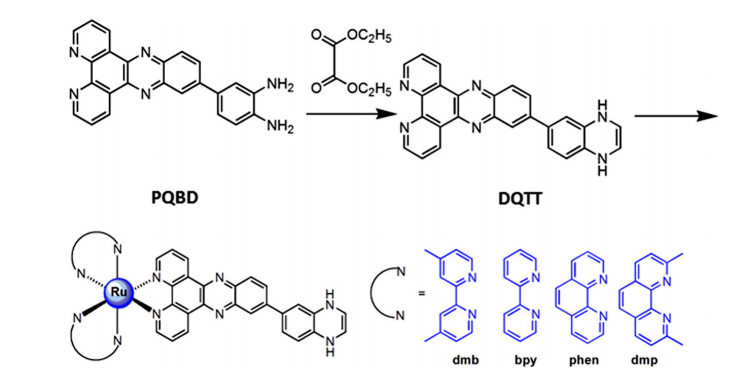
\includegraphics[scale = 0.55]{ruthone.png}
    \caption{The synthetic route of ligand and complexes.}
    \label{fig:ruthone}
\end{figure}

\subsection{Rhodium Complexes}

Rh(III) complexes were considered unlikely agents for anti-cancer agents due to their typical kinetic inertness transition metal centers. High cytotoxicity has been observed for all half-sandwich complexes of the type [(co-ligand)RhCl(pp)]n+ containing the larger polypyridyl ligands dpq and dppz, and it is only the co-ligand [9]aneS3 that "switches on" activity for the smaller bpy ligand \cite{geldmacher2012rhodium}.

Khan et al. synthesized and examined two new rhodium complexes with isoquinoline derivatives. The Figure \ref{fig:rhodone} and \ref{fig:rhodtwo} shows the two rhodium complexes. The authors reported that both complexes exhibited intense anti-cancer activity against various cancer cells and low cytotoxicity against non-cancer cells. The apoptosis of infected cancer cells occurred via mitochondrial dysfunction that increased ROS and \ce{Ca2+} and released cytochrome C, ultimately activated caspases and the apoptosis pathway.  Rh1 displayed a more favorable in vivo safety profile than cisplatin, and the tumor inhibition ratios were comparable. Rh1 is a potential leading compound for further development as an anti-cancer agent. 

\begin{figure}[!ht]
    \centering
    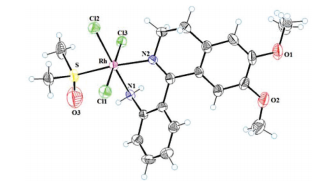
\includegraphics[scale = 1.5]{rodone.png}
    \caption{ORTEP view of the complex Rh1.}
    \label{fig:rhodone}
\end{figure}

\begin{figure}[!ht]
    \centering
    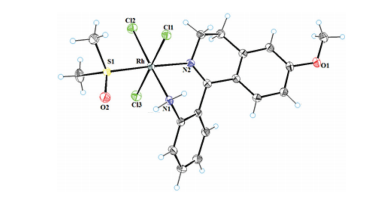
\includegraphics[scale = 1.5]{rodtwo.png}
    \caption{ORTEP view of the complex Rh2.}
    \label{fig:rhodtwo}
\end{figure}


\begin{table}
\begin{tabular}{|l|l|l|l|l|l|} 
\hline
\multirow{2}{*}{Rhodium complex}                     & \multicolumn{5}{l|}{IC\textsubscript{50} values [\SI{}{\micro}M]}                                    \\ 
\cline{2-6}
                                                     & T-24         & ~BEL-7704   & HeLa        & MGC80-3~    & A-549       \\ 
\hline
RH1 & 4.08 ± 0.3   & 18.04 ± 0.3 & 22.02 ± 0.6 & 62.05 ± 0.6 & 75.1 ± 0.9  \\ 
\hline
Rh2 & 10.02 ± 0.8~ & 70.03 ± 0.5 & 59.03 ± 0.1 & 65.7 ± 0.4  & 30.4 ± 0.5  \\ 
\hline
Cisplatin                                            & 27.02 ± 0.3  & 24.03 ± 0.6 & 9.5 ± 0.8   & 8.02 ± 0.8  & 19.9 ± 0.5  \\
\hline
\end{tabular}
\caption{IC\textsubscript{50} values of the proposed rhodium complexes}
\label{tab:rod}
\end{table}

Burgoyne et al. \cite{burgoyne2017synthesis} proposed using mononuclear and trinuclear half-sandwich Rh(III) complexes based on sulfonated scaffolds, and the author evaluated the cytotoxicity against the WHC01 oesophageal cancer cell line. The focus of the study, as mentioned earlier, was to combine the dimeric precursors, [Rh(C5Me5)Cl2]2 and [Ir(C5Me5)Cl2]2 with N,O-salicylaldiminato sulfonated ligands to yield bidentate (N,O-) trinuclear complexes.  The authors observed that the trinuclear complexes tested showed more significant cytotoxicity. Table \ref{tab:rhodvalues} shows the IC\textsubscript{50} values. 


\begin{table}
\centering
\begin{tabular}{|l|l|} 
\hline
\multirow{2}{*}{Rhodium complex}                     & IC\textsubscript{50} values  [\SI{}{\micro}M] \\ 
\cline{2-2}
                                                     & WHCO1             \\ 
\hline
Mononuclear N,O-salicylaldiminato-sulfonated complex & 169.1 ± 13.2      \\ 
\hline
Trinuclear N,O-salicylaldiminato-sulfonated complex & 43.9 ± 31.9       \\ 
\hline
Cisplatin                                            & 9.2 ± 0.1         \\
\hline

\end{tabular}
\caption{IC50 values of the mononuclear and trinuclear rhodium complexes}
\label{tab:rhodvalues}

\end{table}